\documentclass[8pt,aspectratio=169]{beamer}
\usetheme{Boadilla}

\usepackage{hyperref}
\usepackage{graphicx}
\usepackage{subfig}
\usepackage{amsmath,amssymb}

\graphicspath{ {img/} }

\usepackage{tikz}

%Some useful commands for QM
\newcommand{\bra}[1]{\left< #1 \right|}
\newcommand{\ket}[1]{\left| #1 \right>}
\newcommand{\expVal}[1]{\left< #1 \right>}
\newcommand{\braket}[2]{\left<#1|#2\right>}

% Set beamer color info
\definecolor{BOrange}{RGB}{191,87,0}
\setbeamercolor{title}{fg=black}
\setbeamercolor{frametitle}{fg=black}
\setbeamercolor{structure}{fg=BOrange}

%Stolen from http://tex.stackexchange.com/questions/178800/creating-sections-each-with-title-pages-in-beamers-slides
\AtBeginSection[]{
  \begin{frame}
  \vfill
  \centering
  \begin{beamercolorbox}[sep=8pt,center,shadow=true,rounded=true]{title}
    \usebeamerfont{title}\insertsectionhead\par%
  \end{beamercolorbox}
  \vfill
  \end{frame}
}

\title{Holographic Complexity and Volume}
\subtitle{Work with Stefan Eccles, Ted Jacobson, and Phuc Nguyen\\ arxiv:1807.02186}
\author{Josiah Couch}
\institute{University of Texas at Austin}
\date{16 February 2019}



\begin{document}

\begin{frame}
\titlepage

\end{frame}

\begin{frame}
\frametitle{Introducion}

\begin{minipage}[t]{0.44\linewidth}

We would like to study properties of maximal volume slice. Why?

\begin{itemize}

\item Conjectured by Susskind to be dual to circuit complexity of CFT state.

\item Regardless of complexity, can capture growth of wormhole for eternal black hole.

\item New tools brought to like by Freedman and Headrick, Headrick and Hubeny (max-cut/min-flow). 

\end{itemize}

\end{minipage}\hfill
%
\begin{minipage}[t]{0.55\linewidth}

\begin{figure}
    \begin{center}
    
        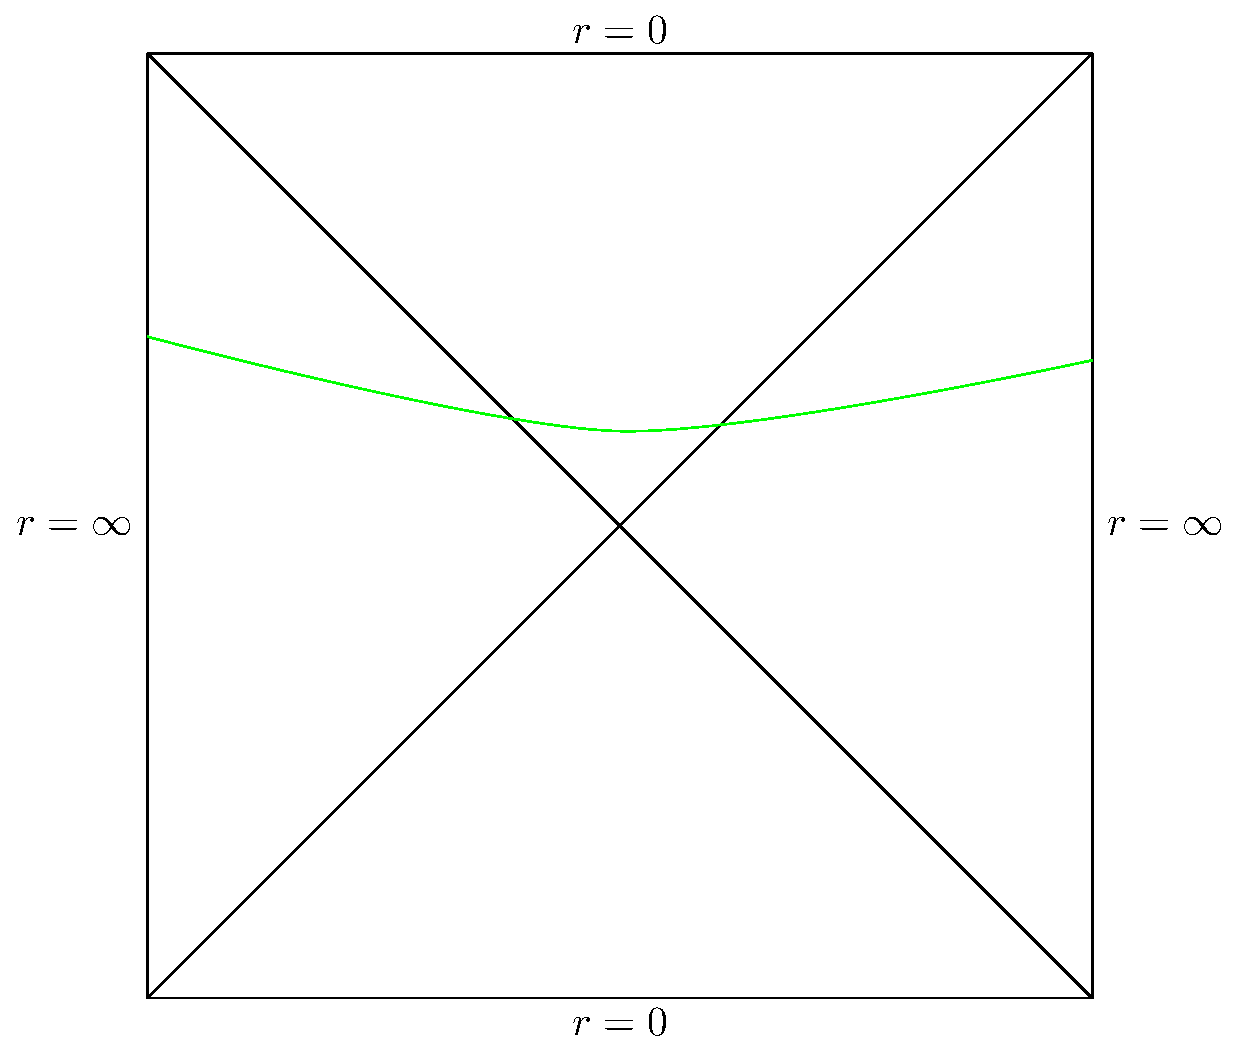
\includegraphics[scale=0.35]{CV}    
    
    \end{center}
    \caption{A maximal spatial slice}
    \label{fig:WDW}
\end{figure}

\end{minipage}

\end{frame}

\begin{frame}
\frametitle{Max-Cut/Min-Flow}

\begin{minipage}[t]{0.55\linewidth}

We are interested in applying ideas similar to the bit-thread ideas of Freedman and Headrick. This makes use of the min-cut/max-flow theorem, by which you can find a maximum flux in place of a minimal area. In Lorentzian signature, this becomes max-cut/min-flow as detailed by Headrick and Hubeny.

\begin{itemize}

\item Let a {\it flow} be a timelike future directed divergence free vector field $v$ such that everywhere in spacetime, $1\leq |v|$.

\item Consider a Lorentzian manifold with a timelike boundary, and let $\sigma$ be a cauchy slice of that boundary.

\item Then the volume of the maximal slice of the bulk bounded by $\sigma$ can be found by finding the minimum over all flows of the flux through {\it any} slice bounded by $\sigma$. 

\item max-cut/min-flow has a {\it nesting property}, namely that given two boundary cauchy slices $\sigma_1$ and $\sigma_2$ such that $sigma_1$ is entirely to the past of $\sigma_2$, then there is a flow (highly non-unique) flow whose flux computes the maximal volumes bounded by both $\sigma_1$ and $\sigma_2$. 

\item In fact, we could have taken an entire boundary foliation.

\end{itemize}

\end{minipage}\hfill
%
\begin{minipage}[t]{0.44\linewidth}

\begin{figure}
    \begin{center}
    
        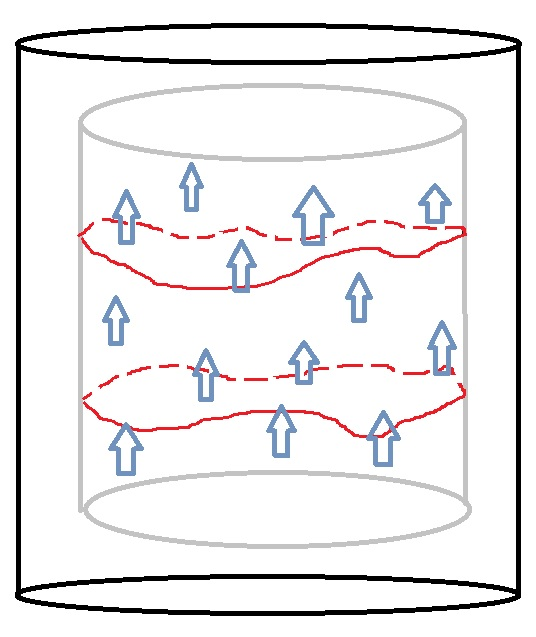
\includegraphics[scale=0.6]{Nesting}    
    
    \end{center}
    \caption{Volume Flow}
    \label{fig:WDW}
\end{figure}

\end{minipage}

\end{frame}

\begin{frame}
\frametitle{Volume Flow}

\begin{minipage}[t]{0.44\linewidth}

\begin{itemize}

\item The flows defined above are in general highly non-unique. 

\item However, whenever a boundary foliation induces a bulk foliation by maximal slices, the unit vector field normal to this bulk foliation is an example of such a flow. 

\item We will focus on this particular flow, which we will call the volume flow. 

\item Question: Does a foliation of the boundary automatically give a foliation of the bulk by maximal slices? 

\item In our paper, we answer yes given Einstein's equation and the strong energy condition.

\end{itemize}

\end{minipage}\hfill
%
\begin{minipage}[t]{0.55\linewidth}

\begin{figure}
    \begin{center}
    
        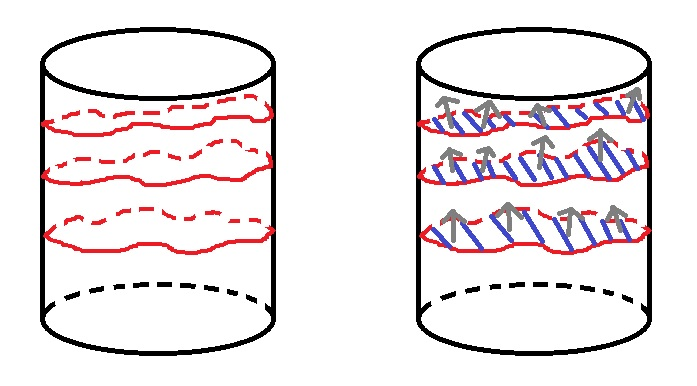
\includegraphics[scale=0.6]{ComplexityFlow}    
    
    \end{center}
    \caption{Foliations}
    \label{fig:WDW}
\end{figure}

\end{minipage}

\end{frame}

\begin{frame}
\frametitle{Insights from Volume Flows}

\begin{minipage}[t]{0.55\linewidth}

What do we learn from these volume flows?

\begin{itemize}

\item In looking at examples, we see that volume seems to flow away from boundary, possibly indicating a flow from UV into IR (of dual theory).

\item In volume language, it is clear that the growth of the wormhole is generic:

	\begin{itemize}

	\item Given any future horizon, volume flow can have an inbound flux but not outbound flux.
	
	\item This is of course a direct consequence of the flow being timelike and future directed.
	
	\item Perhaps reminiscent of the proposed 2nd law of complexity?

	\end{itemize}
	
\item We can also show a monotonicity property for the rate of increase of the maximal volume (in the boundary time).

\end{itemize}

\end{minipage}\hfill
%
\begin{minipage}[t]{0.44\linewidth}

\begin{figure}
    \begin{center}
    
        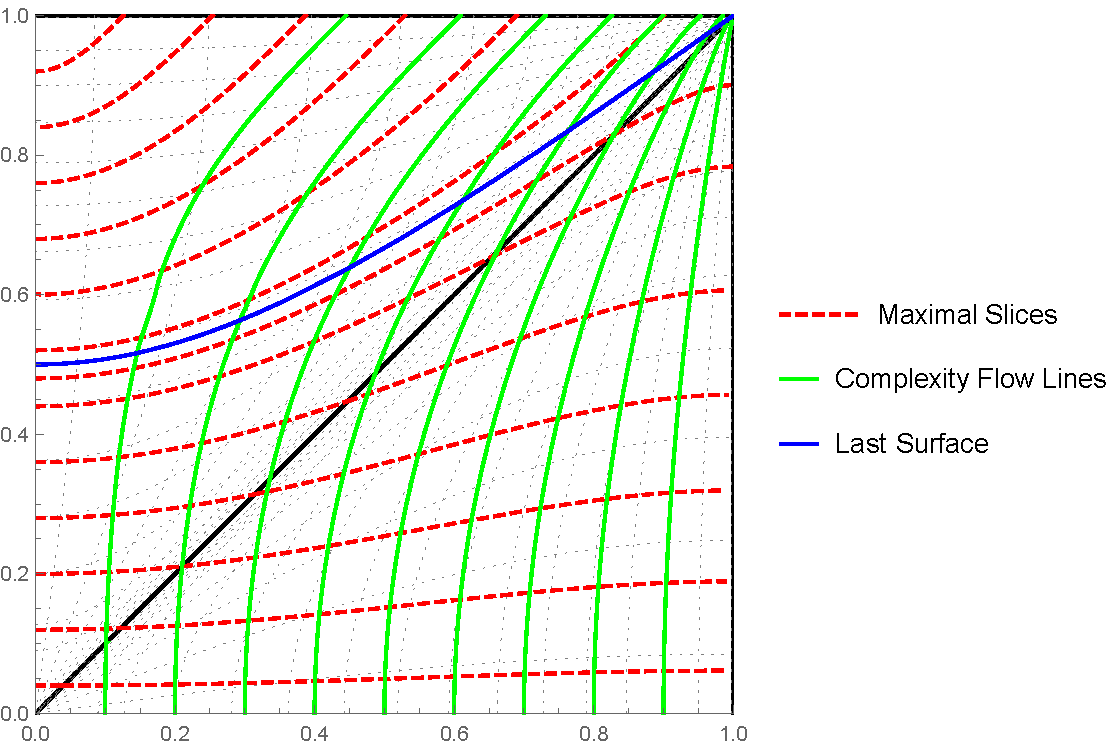
\includegraphics[scale=0.35]{VolumeFlowDisplay}    
    
    \end{center}
    \caption{An example of a volume flow with a future horizon}
    \label{fig:WDW}
\end{figure}

\end{minipage}

\end{frame}

\begin{frame}
\frametitle{A Monotonicity Property}

\begin{minipage}[t]{0.55\linewidth}

\begin{itemize}

\item Consider boundary cauchy slices $\sigma_1$ and $\sigma_2$, and let their union be denoted by $\sigma_U$. 

\item Define $\sigma_+$ to be the set of points $x$ in $\sigma_U$ such that the future of $x$ only intersects $\sigma_U$ at $x$.

\item Likewise define $\sigma_-$ to be the set of points $x$ in $\sigma_U$ such that the past of $x$ only intersects $\sigma_U$ at $x$.

\item Then $\text{Vol}(\sigma_1) + \text{Vol}(\sigma_2) \leq \text{Vol}(\sigma_+) + \text{Vol}(\sigma_-)$

\item We can prove this based on the definition of a maximal slice without reference to flows, but there is a proof of this fact from flows based on their nesting property, which is exactly the Lorentzian analog of the proof of SSA in Freedman and Headrick.

\item Applied to a two sided black hole, this implies that the rate of increase of maximal volume (as you increase the $t_L + t_R$, where both times increase towards the future) is monotonic. 

\end{itemize}

\end{minipage}\hfill
%
\begin{minipage}[t]{0.42\linewidth}

\begin{figure}
    \begin{center}
    
        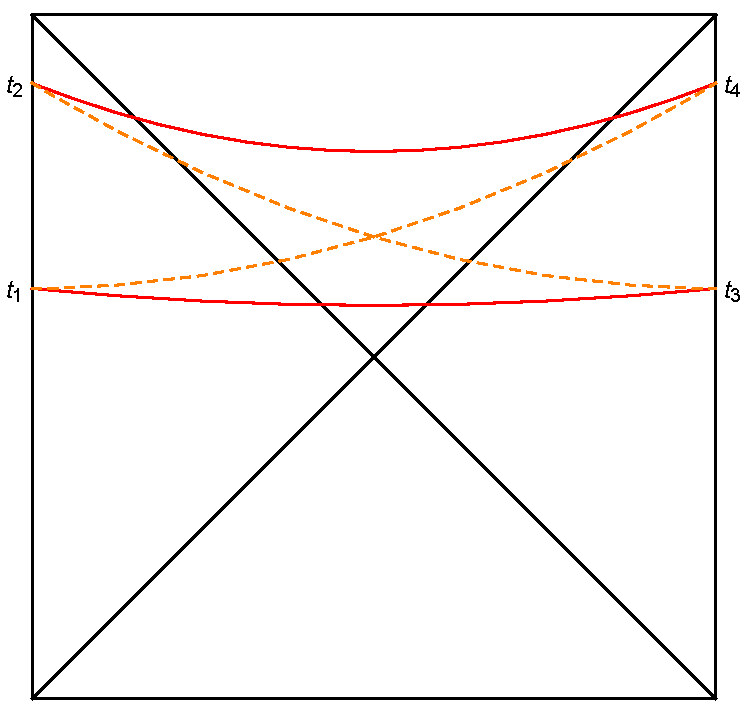
\includegraphics[scale=0.35]{SSA}    
    
    \end{center}
    \caption{Maximal slices associated to different boundary slices for two-sided BH.}
    \label{fig:WDW}
\end{figure}

\end{minipage}

\end{frame}


\begin{frame}
\frametitle{Complexity = Action or Volume?}


\end{frame}



\end{document}